\subsection{Linear Solver}

\def \pepoat {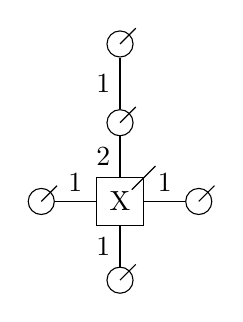
\begin{tikzpicture}[baseline=0.5]

        \def \legLength { 0.8}
        \def \radius {0.1}

        \pgfmathsetmacro{\step}{2*\radius+ \legLength} % 1
        \pgfmathsetmacro{\legpos}{\radius+\legLength} %0.9

        \node[draw,minimum size=0.6cm] (O0) at (0,0) {X};
        \draw (0.15,0.15) -- ++(0.3,0.3);

        \node[draw, circle,radius=\radius] (L1) at (-1,0) {};
        %\node[draw, circle,radius=\radius] (L2) at (-2,0) {};
        %\node[draw, circle,radius=\radius] (L3) at (-3,0) {};

        \node[draw, circle,radius=\radius] (U1) at (0,1) {};
        \node[draw, circle,radius=\radius] (U2) at (0,2) {};

        \node[draw, circle,radius=\radius] (D1) at (0,-1) {};

        \node[draw, circle,radius=\radius] (R1) at (1,0) {};

        \draw (O0) -- node [above] {1}  (L1);
        %\draw (L2) -- node [above] {2}  (L1);
        %\draw (L2) -- node [above] {1}  (L3);

        \draw (O0) -- node [left] {2}  (U1);
        \draw (U2) -- node [left] {1}  (U1);

        \draw (O0) -- node [above] {1}  (R1);

        \draw (O0) --  node [left] {1} (D1);

        \draw (L1.center) -- ++(0.2,0.2);
        %\draw (L2.center) -- ++(0.2,0.2);
        %\draw (L3.center) -- ++(0.2,0.2);
        \draw (U1.center) -- ++(0.2,0.2);
        \draw (U2.center) -- ++(0.2,0.2);
        \draw (R1.center) -- ++(0.2,0.2);
        \draw (D1.center) -- ++(0.2,0.2);

    \end{tikzpicture}}

\def \blockat {  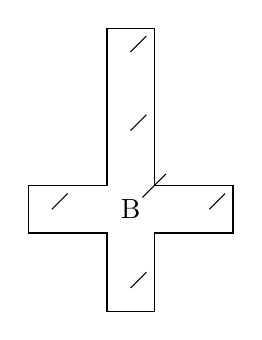
\begin{tikzpicture}[baseline=0.5]

        \def \legLength { 0.8}
        \def \radius {0.1}

        \pgfmathsetmacro{\step}{2*\radius+ \legLength} % 1
        \pgfmathsetmacro{\legpos}{\radius+\legLength} %0.9

        %\node[draw=none] (O0) at (0,0) {};
        \node[draw=none,minimum size=0.6cm] (O0) at (0,0) {B};
        \draw (0.15,0.15) -- ++(0.3,0.3);

        \node[draw=none] (L1) at (-1,0) {};
        %\node[draw=none] (L2) at (-2,0) {};
        %\node[draw=none] (L3) at (-3,0) {};

        \node[draw=none] (U1) at (0,1) {};
        \node[draw=none] (U2) at (0,2) {};

        \node[draw=none] (D1) at (0,-1) {};

        \node[draw=none] (R1) at (1,0) {};

        %\draw (O0.center) -- ++(0.45,0.45);
        \draw (L1.center) -- ++(0.2,0.2);
        %\draw (L2.center) -- ++(0.2,0.2);
        %\draw (L3.center) -- ++(0.2,0.2);
        \draw (U1.center) -- ++(0.2,0.2);
        \draw (U2.center) -- ++(0.2,0.2);
        \draw (R1.center) -- ++(0.2,0.2);
        \draw (D1.center) -- ++(0.2,0.2);

        \draw (-1.3,0.3)--(-0.3,0.3) -- (-0.3,2.3)--(0.3,2.3)
        -- (0.3,0.3) -- (1.3,0.3) -- (1.3,-0.3) -- (0.3,-0.3)
        -- (0.3,-1.3) -- (-0.3, -1.3) -- (-0.3,-0.3) -- (-1.3,-0.3) -- cycle;

    \end{tikzpicture}}

\def \pepobt {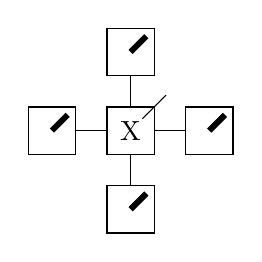
\begin{tikzpicture}[baseline=0.5]

        \def \legLength { 0.8}
        \def \radius {0.1}

        \pgfmathsetmacro{\step}{2*\radius+ \legLength} % 1
        \pgfmathsetmacro{\legpos}{\radius+\legLength} %0.9

        %\node[draw, circle, radius=\radius] (O0) at (0,0) {};
        \node[draw,minimum size=0.6cm] (O0) at (0,0) {X};
        \draw (0.15,0.15) -- ++(0.3,0.3);

        \node[draw, minimum size=0.6cm] (L1) at (-1,0) {};
        \node[draw, minimum size=0.6cm] (U1) at (0,1) {};
        \node[draw, minimum size=0.6cm] (D1) at (0,-1) {};
        \node[draw, minimum size=0.6cm] (R1) at (1,0) {};

        \draw (O0) -- (L1);
        \draw (O0) -- (U1);
        \draw (O0) -- (R1);
        \draw (O0) -- (D1);

        %\draw(O0.center) -- ++(0.2,0.2);
        \draw[line width=0.75mm]  (L1.center) -- ++(0.2,0.2);
        \draw[line width=0.75mm] (U1.center) -- ++(0.2,0.2);
        \draw[line width=0.75mm] (R1.center) -- ++(0.2,0.2);
        \draw[line width=0.75mm] (D1.center) -- ++(0.2,0.2);

    \end{tikzpicture} }

\def \blockbt {   \begin{tikzpicture}[baseline=0.5]

        \def \legLength { 0.8}
        \def \radius {0.1}

        \pgfmathsetmacro{\step}{2*\radius+ \legLength} % 1
        \pgfmathsetmacro{\legpos}{\radius+\legLength} %0.9

        %\node[draw=none] (O0) at (0,0) {};
        \node[draw=none,minimum size=0.6cm] (O0) at (0,0) {B};
        \draw (0.15,0.15) -- ++(0.3,0.3);

        \node[draw=none] (L1) at (-1,0) {};
        \node[draw=none] (L2) at (-2,0) {};
        \node[draw=none] (L3) at (-3,0) {};

        \node[draw=none] (U1) at (0,1) {};
        \node[draw=none] (U2) at (0,2) {};

        \node[draw=none] (D1) at (0,-1) {};

        \node[draw=none] (R1) at (1,0) {};

        %\draw (O0.center) -- ++(0.45,0.45);
        \draw[line width=0.75mm] (L3.center) -- ++(0.2,0.2);
        \draw[line width=0.75mm] (U2.center) -- ++(0.2,0.2);
        \draw[line width=0.75mm] (R1.center) -- ++(0.2,0.2);
        \draw[line width=0.75mm] (D1.center) -- ++(0.2,0.2);

        \draw (-3.3,0.3)--(-0.3,0.3) -- (-0.3,2.3)--(0.3,2.3)
        -- (0.3,0.3) -- (1.3,0.3) -- (1.3,-0.3) -- (0.3,-0.3)
        -- (0.3,-1.3) -- (-0.3, -1.3) -- (-0.3,-0.3) -- (-3.3,-0.3) -- cycle;

    \end{tikzpicture} }

\def \pepoct { 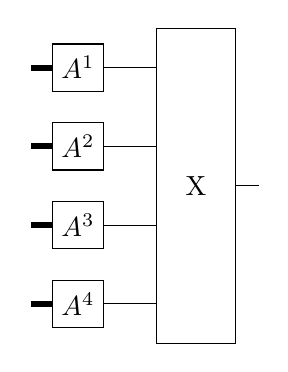
\begin{tikzpicture}[baseline=0.5]
        \draw (0,2.5)-- (0,-1.5) -- (1,-1.5)-- (1,2.5) -- cycle;

        \node[draw=none] (x)  at (0.5,0.5) {X};

        \node[draw, minimum size=0.6cm] (n1)  at (-1,2) {$A^1$};
        \node[draw, minimum size=0.6cm] (n2)  at (-1,1) {$A^2$};
        \node[draw, minimum size=0.6cm] (n3)  at (-1,0) {$A^3$};
        \node[draw, minimum size=0.6cm] (n4)  at (-1,-1) {$A^4$};

        \draw (n1) -- node [above] {} (0,2);
        \draw (n2) -- node [above] {} (0,1);
        \draw (n3) -- node [above] {} (0,0);
        \draw (n4) -- node [above] {} (0,-1);

        \draw[line width=0.75mm] (n1) -- ++(-0.6,0) ;
        \draw[line width=0.75mm] (n2) -- ++(-0.6,0) ;
        \draw[line width=0.75mm] (n3) -- ++(-0.6,0) ;
        \draw[line width=0.75mm] (n4) -- ++(-0.6,0);

        \draw (1,0.5) -- (1.3,0.5)  ;

    \end{tikzpicture} }

\def \blockct { \begin{tikzpicture}[baseline=3]
        \draw (0,2.5)-- (0,-1.5) -- (1,-1.5)-- (1,2.5) -- cycle;

        \node[draw=none] (x)  at (0.5,0.5) {B};

        \draw[line width=0.75mm] (-0.3,2)  node [left] {}  -- (0,2) ;
        \draw[line width=0.75mm] (-0.3,1)  node [left] {} -- (0,1);
        \draw[line width=0.75mm] (-0.3,0)  node [left] {} -- (0,0);
        \draw[line width=0.75mm] (-0.3,-1)  node [left] {} -- (0,-1);

        \draw (1,0.5) -- (1.3,0.5)  node [right] {} ;

    \end{tikzpicture} }

\def \pepocta { 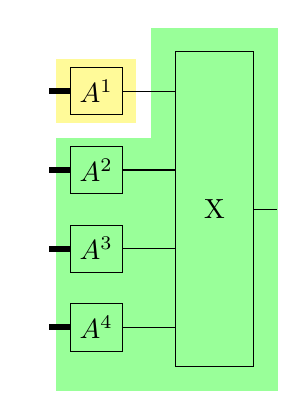
\begin{tikzpicture}[baseline=0.5]

        \path[draw, fill=yellow!40,color=yellow!40] (-1.5,2.4) -- (-0.5,2.4)--(-0.5,1.6)--(-1.5,1.6)-- cycle;

        \path[draw, fill=green!40,color=green!40] (-1.5,1.4) -- (-0.3,1.4)--(-0.3,2.8)--(1.3,2.8)-- (1.3,-1.8) -- (-1.5 ,-1.8) -- cycle;

        \draw (0,2.5)-- (0,-1.5) -- (1,-1.5)-- (1,2.5) -- cycle;

        \node[draw=none] (x)  at (0.5,0.5) {X};

        \node[draw, minimum size=0.6cm] (n1)  at (-1,2) {$A^1$};
        \node[draw, minimum size=0.6cm] (n2)  at (-1,1) {$A^2$};
        \node[draw, minimum size=0.6cm] (n3)  at (-1,0) {$A^3$};
        \node[draw, minimum size=0.6cm] (n4)  at (-1,-1) {$A^4$};

        \draw (n1) -- node [above] {} (0,2);
        \draw (n2) -- node [above] {} (0,1);
        \draw (n3) -- node [above] {} (0,0);
        \draw (n4) -- node [above] {} (0,-1);

        \draw[line width=0.75mm] (n1) -- ++(-0.6,0) node [left] {};
        \draw[line width=0.75mm] (n2) -- ++(-0.6,0) node [left] {};
        \draw[line width=0.75mm] (n3) -- ++(-0.6,0) node [left] {};
        \draw[line width=0.75mm] (n4) -- ++(-0.6,0) node [left] {};

        \draw (1,0.5) -- (1.3,0.5)  ;

    \end{tikzpicture} }

\def \blockcta { 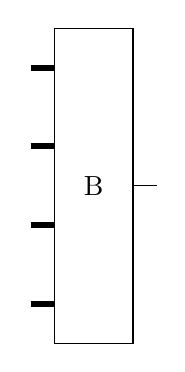
\begin{tikzpicture}[baseline=3]
        \draw (0,2.5)-- (0,-1.5) -- (1,-1.5)-- (1,2.5) -- cycle;

        \node[draw=none] (x)  at (0.5,0.5) {B};

        \draw[line width=0.75mm] (-0.3,2)   -- (0,2) ;
        \draw[line width=0.75mm] (-0.3,1)  -- (0,1);
        \draw[line width=0.75mm] (-0.3,0)   -- (0,0);
        \draw[line width=0.75mm] (-0.3,-1)  -- (0,-1);

        \draw (1,0.5) -- (1.3,0.5)   ;

    \end{tikzpicture} }

\def \pepoctb { 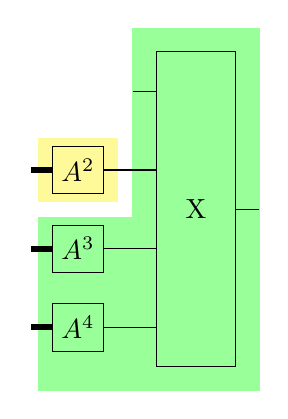
\begin{tikzpicture}[baseline=0.5]

        \path[draw, fill=yellow!40,color=yellow!40] (-1.5,1.4) -- (-0.5,1.4)--(-0.5,0.6)--(-1.5,0.6)-- cycle;

        \path[draw, fill=green!40,color=green!40] (-1.5,0.4) -- (-0.3,0.4)--(-0.3,2.8)--(1.3,2.8)-- (1.3,-1.8) -- (-1.5 ,-1.8) -- cycle;

        \draw (0,2.5)-- (0,-1.5) -- (1,-1.5)-- (1,2.5) -- cycle;

        \node[draw=none] (x)  at (0.5,0.5) {X};

        \node[draw, minimum size=0.6cm] (n2)  at (-1,1) {$A^2$};
        \node[draw, minimum size=0.6cm] (n3)  at (-1,0) {$A^3$};
        \node[draw, minimum size=0.6cm] (n4)  at (-1,-1) {$A^4$};

        \draw (-0.3,2) -- node [above] {} (0,2);
        \draw (n2) -- node [above] {} (0,1);
        \draw (n3) -- node [above] {} (0,0);
        \draw (n4) -- node [above] {} (0,-1);

        \draw[line width=0.75mm] (n2) -- ++(-0.6,0) ;
        \draw[line width=0.75mm] (n3) -- ++(-0.6,0) ;
        \draw[line width=0.75mm] (n4) -- ++(-0.6,0) ;

        \draw (1,0.5) -- (1.3,0.5)  ;

    \end{tikzpicture} }

\def \blockctb { 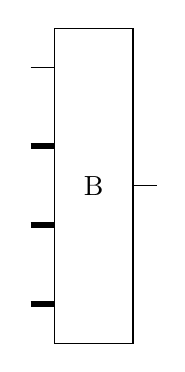
\begin{tikzpicture}[baseline=3]
        \draw (0,2.5)-- (0,-1.5) -- (1,-1.5)-- (1,2.5) -- cycle;

        \node[draw=none] (x)  at (0.5,0.5) {B};

        \draw (-0.3,2)    -- (0,2) ;
        \draw[line width=0.75mm] (-0.3,1)   -- (0,1);
        \draw[line width=0.75mm] (-0.3,0)   -- (0,0);
        \draw[line width=0.75mm] (-0.3,-1)  -- (0,-1);

        \draw (1,0.5) -- (1.3,0.5)  ;

    \end{tikzpicture} }

\def \pepoctc { 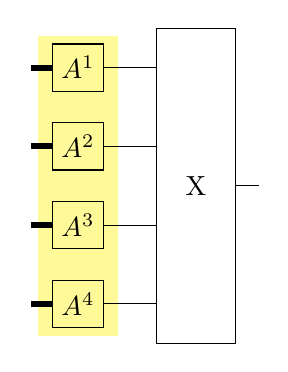
\begin{tikzpicture}[baseline=0.5]

        \path[draw, fill=yellow!40,color=yellow!40] (-1.5,2.4) -- (-0.5,2.4)--(-0.5,-1.4)--(-1.5,-1.4)-- cycle;

        \draw (0,2.5)-- (0,-1.5) -- (1,-1.5)-- (1,2.5) -- cycle;

        \node[draw=none] (x)  at (0.5,0.5) {X};

        \node[draw, minimum size=0.6cm] (n1)  at (-1,2) {$A^1$};
        \node[draw, minimum size=0.6cm] (n2)  at (-1,1) {$A^2$};
        \node[draw, minimum size=0.6cm] (n3)  at (-1,0) {$A^3$};
        \node[draw, minimum size=0.6cm] (n4)  at (-1,-1) {$A^4$};

        \draw (n1) -- node [above] {} (0,2);
        \draw (n2) -- node [above] {} (0,1);
        \draw (n3) -- node [above] {} (0,0);
        \draw (n4) -- node [above] {} (0,-1);

        \draw[line width=0.75mm] (n1) -- ++(-0.6,0) ;
        \draw[line width=0.75mm] (n2) -- ++(-0.6,0) ;
        \draw[line width=0.75mm] (n3) -- ++(-0.6,0) ;
        \draw[line width=0.75mm] (n4) -- ++(-0.6,0) ;

        \draw (1,0.5) -- (1.3,0.5)  ;

    \end{tikzpicture} }

\def \pepoctd{ 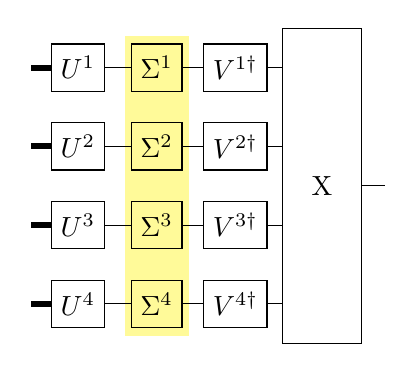
\begin{tikzpicture}[baseline=0.5]

        \path[draw, fill=yellow!40,color=yellow!40] (-2.0,2.4) -- (-1.2,2.4)--(-1.2,-1.4)--(-2.0,-1.4)-- cycle;

        \draw (0,2.5)-- (0,-1.5) -- (1,-1.5)-- (1,2.5) -- cycle;

        \node[draw=none] (x)  at (0.5,0.5) {X};

        \node[draw, minimum size=0.6cm] (n11)  at (-2.6,2) {$U^1$};
        \node[draw, minimum size=0.6cm] (n12)  at (-1.6,2) {$\Sigma^1$};
        \node[draw, minimum size=0.6cm] (n13)  at (-0.6,2) {$V^{1 \dagger}$};

        \node[draw, minimum size=0.6cm] (n21)  at (-2.6,1) {$U^2$};
        \node[draw, minimum size=0.6cm] (n22)  at (-1.6,1) {$\Sigma^2$};
        \node[draw, minimum size=0.6cm] (n23)  at (-0.6,1) {$V^{2 \dagger}$};

        \node[draw, minimum size=0.6cm] (n31)  at (-2.6,0) {$U^3$};
        \node[draw, minimum size=0.6cm] (n32)  at (-1.6,0) {$\Sigma^3$};
        \node[draw, minimum size=0.6cm] (n33)  at (-0.6,0) {$V^{3 \dagger}$};

        \node[draw, minimum size=0.6cm] (n41)  at (-2.6,-1) {$U^4$};
        \node[draw, minimum size=0.6cm] (n42)  at (-1.6,-1) {$\Sigma^4$};
        \node[draw, minimum size=0.6cm] (n43)  at (-0.6,-1) {$V^{4 \dagger}$};

        \draw (n12) --  (n13);
        \draw (n11) --  (n12);

        \draw (n22) --  (n23);
        \draw (n21) --  (n22);

        \draw (n32) --  (n33);
        \draw (n31) --  (n32);

        \draw (n42) --  (n43);
        \draw (n41) --  (n42);

        \draw (n13) -- node [above] {} (0,2);
        \draw (n23) -- node [above] {} (0,1);
        \draw (n33) -- node [above] {} (0,0);
        \draw (n43) -- node [above] {} (0,-1);

        \draw[line width=0.75mm] (n11) -- ++(-0.6,0) ;
        \draw[line width=0.75mm] (n21) -- ++(-0.6,0) ;
        \draw[line width=0.75mm] (n31) -- ++(-0.6,0) ;
        \draw[line width=0.75mm] (n41) -- ++(-0.6,0) ;

        \draw (1,0.5) -- (1.3,0.5)  ;

    \end{tikzpicture} }

% \begin{frame}{Linear Solver: Standard Form}

%     \begin{minipage}{0.4\textwidth}
%         \begin{equation}
%             \scalebox{0.9}{ \pepoat } \;  =  \; \scalebox{0.9}{\blockat}
%         \end{equation}
%     \end{minipage}
%     \begin{minipage}{0.59\textwidth}
%         \begin{equation}

%         \end{equation}
%     \end{minipage}

%     % \begin{equation}
%     %     % \only<1>{ \vcenter{\hbox{ \pepob{5}{5}{{
%     %     %                         "-","-","-","-",
%     %     %                         "-","-","-","-",
%     %     %                         "1","2","3","1",
%     %     %                         "-","-","-","-",
%     %     %                         "-","-","-","-"}}{{
%     %     %                         "-","-","-","-",
%     %     %                         "-","-","-","-",
%     %     %                         "-","-","-","-",
%     %     %                         "-","1","2","1",
%     %     %                         "-","-","-","-"}}{{
%     %     %                         1,1,1,1,1,
%     %     %                         1,1,1,0,1,
%     %     %                         0,0,0,0,0,
%     %     %                         1,1,1,0,1,
%     %     %                         1,1,1,0,1}} }} }
%     %     \only<1>{  \pepoat \;  =  \;\blockat  }
%     %     %\only<2>{ \pepobt \;  =  \;\blockbt }
%     %     \only<2>{ \vcenter{\hbox{ \pepoct }}  =\vcenter{\hbox{  \blockct }} }
%     % \end{equation}
% \end{frame}

\begin{frame}{Linear Solver: Inversion Scheme}

    \begin{minipage}{0.4\textwidth}
        \only<1> { \begin{equation}
                \scalebox{0.9}{ \pepoat } \;  =  \; \scalebox{0.9}{\blockat}
            \end{equation}}
        \only<2-> {
            \begin{itemize}
                \only<2-> {\item Invert $A^i$ separately }
                      \only<2-3>{
                          \begin{itemize}
                              \item Fast
                              \item Numerically unstable
                          \end{itemize}
                      }
                      \only<4-> { \item Full inversion }
                      \only<4>{
                          \begin{itemize}
                              \item Slow
                              \item Stable for pseudoinverse
                          \end{itemize}
                      }
                      \only<5-> { \item Sparse full inversion }
                      \only<5>{
                          \begin{itemize}
                              \item $A^i = U^i \Sigma^i V^{i\dagger}$
                          \end{itemize}
                      }
            \end{itemize}
        }
    \end{minipage}
    \begin{minipage}{0.59\textwidth}
        \begin{equation}
            \only<1>  {  \vcenter{\hbox{   \scalebox{0.9}{  \pepoct }} } = \vcenter{\hbox{ \scalebox{0.9}{ \blockcta} }} }
            \only<2> { \vcenter{\hbox{  \scalebox{0.9}{  \pepocta } }}  =\vcenter{\hbox{ \scalebox{0.9}{  \blockcta }} }  }
            \only<3> { \vcenter{\hbox{ \scalebox{0.9}{  \pepoctb }}}  =\vcenter{\hbox{ \scalebox{0.9}{  \blockctb }} } }
            \only<4> { \vcenter{\hbox{ \scalebox{0.9}{  \pepoctc } }}  =\vcenter{\hbox{ \scalebox{0.9}{  \blockcta }} } }
            \only<5> { \vcenter{\hbox{\scalebox{0.9}{  \pepoctd }}}  =\vcenter{\hbox{ \scalebox{0.9}{  \blockcta }} } }
        \end{equation}
    \end{minipage}

\end{frame}

% \begin{frame}{Linear Solver: Inversion Scheme}

%     \begin{itemize}
%         \only<1-> {\item Invert $A^i$ separately }
%               \only<1>{
%                   \begin{itemize}
%                       \item Fast
%                       \item Numerically unstable
%                   \end{itemize}
%               }
%               \only<2-> { \item Full inversion $A = A^1 \otimes A^2 \cdots \otimes A^m$ }
%               \only<2>{
%                   \begin{itemize}
%                       \item Slow
%                       \item Stable for pseudoinverse
%                   \end{itemize}
%               }
%               \only<3-> { \item Sparse full inversion }
%               \only<3>{
%                   \begin{itemize}
%                       \item $A^i = U \Sigma V^{\dagger}$
%                       \item $S = S^1 \otimes S^2 \cdots \otimes S^m$
%                   \end{itemize}
%               }
%     \end{itemize}

% \end{frame}

\def \figa { \vcenter{\hbox{ \pepob{5}{3}{{
                        "","","","",
                        "","","","",
                        "","","",""}}{{
                        "","",
                        "","",
                        "","",
                        "","",
                        "",""}}{{
                        1,1,1,1,1,
                        1,0,0,0,1,
                        1,0,0,0,1}} } }}

\def \figb { \vcenter{\hbox{  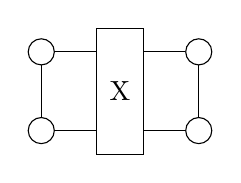
\begin{tikzpicture}[baseline=0.5]

                \def \legLength { 0.8}
                \def \radius {0.1}

                \pgfmathsetmacro{\step}{2*\radius+ \legLength} % 1
                \pgfmathsetmacro{\legpos}{\radius+\legLength} %0.9

                \node[draw, circle,radius=\radius] (L0) at (-1,0) {};
                \node[draw, circle,radius=\radius] (L1) at (-1,1) {};

                \draw (-0.3,1.3) -- (0.3,1.3) -- (0.3,-0.3) -- (-0.3,-0.3) -- cycle;

                \node[draw, circle,radius=\radius] (R0) at (1,0) {};
                \node[draw, circle,radius=\radius] (R1) at (1,1) {};

                \draw (L0) --   (L1);
                \draw (R0) --   (R1);

                \draw (L0) --   (-0.3,0);
                \draw (L1) --   (-0.3,1);

                \draw (R0) --   (0.3,0);
                \draw (R1) --   (0.3,1);

                \node[draw=none] (C0) at (0,0.5) {X};
            \end{tikzpicture}}}}

\def \figc {\vcenter{\hbox{  \begin{tikzpicture}[baseline=0.5]

                \def \legLength { 0.8}
                \def \radius {0.1}

                \pgfmathsetmacro{\step}{2*\radius+ \legLength} % 1
                \pgfmathsetmacro{\legpos}{\radius+\legLength} %0.9

                \node[draw=none, circle,radius=\radius] (L0) at (-1,0) {};
                \node[draw=none, circle,radius=\radius] (L1) at (-1,1) {};

                \draw (-0.3,1.3) -- (0.3,1.3) -- (0.3,-0.3) -- (-0.3,-0.3) -- cycle;

                \node[draw=none, circle,radius=\radius] (R0) at (1,0) {};
                \node[draw=none, circle,radius=\radius] (R1) at (1,1) {};

                \draw (L0) --   (-0.3,0);
                \draw (L1) --   (-0.3,1);

                \draw (R0) --   (0.3,0);
                \draw (R1) --   (0.3,1);

                \node[draw=none] (C0) at (0,0.5) {X};
            \end{tikzpicture} }} }

\def \figd {\vcenter{\hbox{  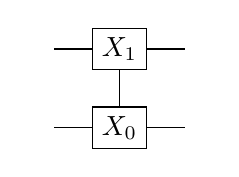
\begin{tikzpicture}[baseline=0.5]

                \def \legLength { 0.8}
                \def \radius {0.1}

                \pgfmathsetmacro{\step}{2*\radius+ \legLength} % 1
                \pgfmathsetmacro{\legpos}{\radius+\legLength} %0.9

                \node[draw=none, circle,radius=\radius] (L0) at (-1,0) {};
                \node[draw=none, circle,radius=\radius] (L1) at (-1,1) {};

                \node[draw] (C0) at (0,0) {$X_0$};
                \node[draw] (C1) at (0,1) {$X_1$};

                \node[draw=none, circle,radius=\radius] (R0) at (1,0) {};
                \node[draw=none, circle,radius=\radius] (R1) at (1,1) {};

                \draw (L0) --   (C0);
                \draw (L1) --   (C1);

                \draw (R0) --   (C0);
                \draw (R1) --   (C1);

                \draw (C1) --   (C0);
            \end{tikzpicture} }}}

\begin{frame}{Linear Solver: Applicability}

    \begin{minipage}{.4\textwidth}
        \begin{equation}
            \vcenter{\hbox{  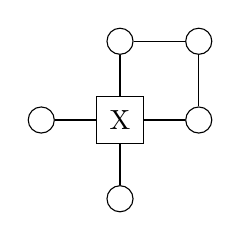
\begin{tikzpicture}[baseline=0.5]

                        \def \legLength { 0.8}
                        \def \radius {0.1}

                        \pgfmathsetmacro{\step}{2*\radius+ \legLength} % 1
                        \pgfmathsetmacro{\legpos}{\radius+\legLength} %0.9

                        \node[draw, circle,radius=\radius] (L0) at (-1,0) {};

                        \draw (-0.3,0.3) -- (0.3,0.3) -- (0.3,-0.3) -- (-0.3,-0.3) -- cycle;

                        \node[draw, circle,radius=\radius] (R0) at (1,0) {};
                        \node[draw, circle,radius=\radius] (R1) at (1,1) {};

                        \node[draw, circle,radius=\radius] (U) at (0,1) {};
                        \node[draw, circle,radius=\radius] (D) at (0,-1) {};

                        \draw (R0) --   (R1);

                        \draw (L0) --   (-0.3,0);

                        \draw (R0) --   (0.3,0);
                        \draw (U) --   (0,0.3);
                        \draw (D) --   (0,-0.3);
                        \draw (R1) --   (U);

                        \node[draw=none] (C0) at (0,0) {X};
                    \end{tikzpicture} }}
        \end{equation}
    \end{minipage}
    \begin{minipage}{.59\textwidth}
        % \begin{equation}
        %     \figa
        % \end{equation}

        \begin{subequations}
            \begin{align}
                 & \figb          \\
                 & \figc =  \figd
            \end{align}
        \end{subequations}
    \end{minipage}

\end{frame}

% \begin{frame}{Linear Solver: Applicability}
%     \begin{equation}
%         \figa
%     \end{equation}

%     \begin{subequations}
%         \begin{align}
%              & \figb          \\
%              & \figc =  \figd
%         \end{align}
%     \end{subequations}
% \end{frame}

\subsection{Nonlinear Solver}
\begin{frame}{Nonlinear Solver}

    \begin{minipage}{0.5\textwidth}
        \begin{itemize}
            \item Nonlinear least squares
            \item Jacobian
            \item Permutations
        \end{itemize}
    \end{minipage}
    \begin{minipage}{0.49\textwidth}
        \begin{equation}
            \vcenter{\hbox{   {\pepob{2}{2}{{"$\alpha$","$\alpha$",}}{{"$\alpha$","$\alpha$",}}{{0,0,0,0}}} }}
        \end{equation}
    \end{minipage}

\end{frame}

\subsection{Sequential Linear Solver}
\begin{frame}{Sequential Linear Solver}
    \begin{itemize}
        \item Based on linear solver
        \item Sweep over unknown tensors
        \item Permutations
    \end{itemize}
\end{frame}